\section{Results}
\label{sec:results}

\begin{table*}[t]
\centering
\small
\setlength{\tabcolsep}{4pt}
\caption{Paired makespan ratio ALNS / competitor (mean over the instances with bootstrap 95\% CI; below 1: ALNS better). $^\dagger$: not significant after Holm's correction (one-sided paired $t$-test on log ratios, $\alpha = 0.05$). CTAS-D failures count as makespan 200; the share of instances it solved within the budget follows its ratio in parentheses; it is not run on the 500-task settings.}
\label{tab:ratios}
\begin{tabular}{lcccccc}
\toprule
Setting & CP-SAT LNS & Par.\ CP-SAT LNS & CP-SAT model & CTAS-D & Restarts & RL(s.$N$) \\
\midrule
\multicolumn{7}{l}{\emph{(a) C1: ALNS on 8 cores vs.\ each competitor on 8 cores, both at budget $B_1$}} \\
SA-BT 25/5/50 & 0.911 {\scriptsize [0.90, 0.92]} & 0.925 {\scriptsize [0.91, 0.93]} & 0.910 {\scriptsize [0.90, 0.92]} & 0.150 {\scriptsize [0.13, 0.19]} (10\%) & 0.919 {\scriptsize [0.91, 0.93]} & 0.799 {\scriptsize [0.78, 0.82]} \\
SA-BT 50/5/50 & 0.968 {\scriptsize [0.96, 0.98]} & 0.951 {\scriptsize [0.94, 0.96]} & 0.930 {\scriptsize [0.92, 0.94]} & 0.538 {\scriptsize [0.51, 0.56]} (100\%) & 0.918 {\scriptsize [0.91, 0.93]} & 0.758 {\scriptsize [0.74, 0.77]} \\
SA-AT 50/5/50 & 0.923 {\scriptsize [0.92, 0.93]} & 0.926 {\scriptsize [0.92, 0.93]} & 0.922 {\scriptsize [0.92, 0.92]} & 0.135 {\scriptsize [0.13, 0.14]} (0\%) & 0.934 {\scriptsize [0.93, 0.94]} & 0.770 {\scriptsize [0.76, 0.78]} \\
MA-AT 25/5/50 & 0.900 {\scriptsize [0.89, 0.91]} & 0.889 {\scriptsize [0.87, 0.90]} & 0.888 {\scriptsize [0.87, 0.90]} & 0.152 {\scriptsize [0.13, 0.18]} (0\%) & 0.903 {\scriptsize [0.89, 0.92]} & 0.733 {\scriptsize [0.71, 0.76]} \\
MA-AT 50/5/50 & 0.890 {\scriptsize [0.87, 0.91]} & 0.907 {\scriptsize [0.90, 0.92]} & 0.877 {\scriptsize [0.86, 0.89]} & 0.127 {\scriptsize [0.09, 0.19]} (10\%) & 0.890 {\scriptsize [0.87, 0.91]} & 0.727 {\scriptsize [0.69, 0.76]} \\
MA-AT 50/5/200 & 0.900 {\scriptsize [0.88, 0.92]} & 0.904 {\scriptsize [0.89, 0.92]} & 0.886 {\scriptsize [0.87, 0.90]} & 0.305 {\scriptsize [0.27, 0.34]} (0\%) & 0.885 {\scriptsize [0.87, 0.90]} & 0.722 {\scriptsize [0.71, 0.74]} \\
MA-AT 150/10/500 & 0.885 {\scriptsize [0.87, 0.90]} & 0.890 {\scriptsize [0.88, 0.91]} & 0.870 {\scriptsize [0.86, 0.89]} & -- & 0.888 {\scriptsize [0.88, 0.90]} & 0.680 {\scriptsize [0.67, 0.69]} \\
MA-AT 150/5/500 & 0.890 {\scriptsize [0.85, 0.94]} & 0.890 {\scriptsize [0.85, 0.93]} & 0.867 {\scriptsize [0.82, 0.91]} & -- & 0.888 {\scriptsize [0.86, 0.92]} & 0.713 {\scriptsize [0.70, 0.73]} \\
\midrule
\multicolumn{7}{l}{\emph{(b) C2: ALNS on 1 core for 2\,s vs.\ each competitor on 8 cores at $B_1$}} \\
SA-BT 25/5/50 & 0.949 {\scriptsize [0.93, 0.96]} & 0.965 {\scriptsize [0.95, 0.98]} & 0.949 {\scriptsize [0.94, 0.96]} & 0.157 {\scriptsize [0.14, 0.19]} (10\%) & 0.958 {\scriptsize [0.94, 0.97]} & 0.833 {\scriptsize [0.82, 0.84]} \\
SA-BT 50/5/50 & 0.995$^\dagger$ {\scriptsize [0.98, 1.01]} & 0.977$^\dagger$ {\scriptsize [0.96, 0.99]} & 0.956 {\scriptsize [0.94, 0.97]} & 0.553 {\scriptsize [0.53, 0.58]} (100\%) & 0.944 {\scriptsize [0.93, 0.96]} & 0.779 {\scriptsize [0.76, 0.80]} \\
SA-AT 50/5/50 & 0.984$^\dagger$ {\scriptsize [0.97, 1.00]} & 0.987$^\dagger$ {\scriptsize [0.97, 1.00]} & 0.982$^\dagger$ {\scriptsize [0.97, 0.99]} & 0.144 {\scriptsize [0.14, 0.15]} (0\%) & 0.995$^\dagger$ {\scriptsize [0.99, 1.00]} & 0.820 {\scriptsize [0.81, 0.83]} \\
MA-AT 25/5/50 & 0.938 {\scriptsize [0.93, 0.95]} & 0.927 {\scriptsize [0.91, 0.94]} & 0.925 {\scriptsize [0.91, 0.94]} & 0.158 {\scriptsize [0.14, 0.18]} (0\%) & 0.941 {\scriptsize [0.93, 0.95]} & 0.764 {\scriptsize [0.75, 0.78]} \\
MA-AT 50/5/50 & 0.934 {\scriptsize [0.91, 0.95]} & 0.952 {\scriptsize [0.93, 0.97]} & 0.920 {\scriptsize [0.90, 0.94]} & 0.133 {\scriptsize [0.09, 0.20]} (10\%) & 0.934 {\scriptsize [0.91, 0.95]} & 0.762 {\scriptsize [0.73, 0.79]} \\
MA-AT 50/5/200 & 0.949 {\scriptsize [0.93, 0.96]} & 0.954 {\scriptsize [0.94, 0.97]} & 0.935 {\scriptsize [0.92, 0.95]} & 0.321 {\scriptsize [0.28, 0.36]} (0\%) & 0.933 {\scriptsize [0.92, 0.95]} & 0.762 {\scriptsize [0.75, 0.78]} \\
MA-AT 150/10/500 & 0.980 {\scriptsize [0.97, 0.99]} & 0.986 {\scriptsize [0.98, 0.99]} & 0.964 {\scriptsize [0.96, 0.97]} & -- & 0.983$^\dagger$ {\scriptsize [0.97, 0.99]} & 0.753 {\scriptsize [0.74, 0.76]} \\
MA-AT 150/5/500 & 0.960$^\dagger$ {\scriptsize [0.93, 0.99]} & 0.960$^\dagger$ {\scriptsize [0.94, 0.98]} & 0.935 {\scriptsize [0.91, 0.96]} & -- & 0.958 {\scriptsize [0.94, 0.97]} & 0.771 {\scriptsize [0.74, 0.79]} \\
\bottomrule
\end{tabular}
\end{table*}


\begin{figure*}[t]
\centering
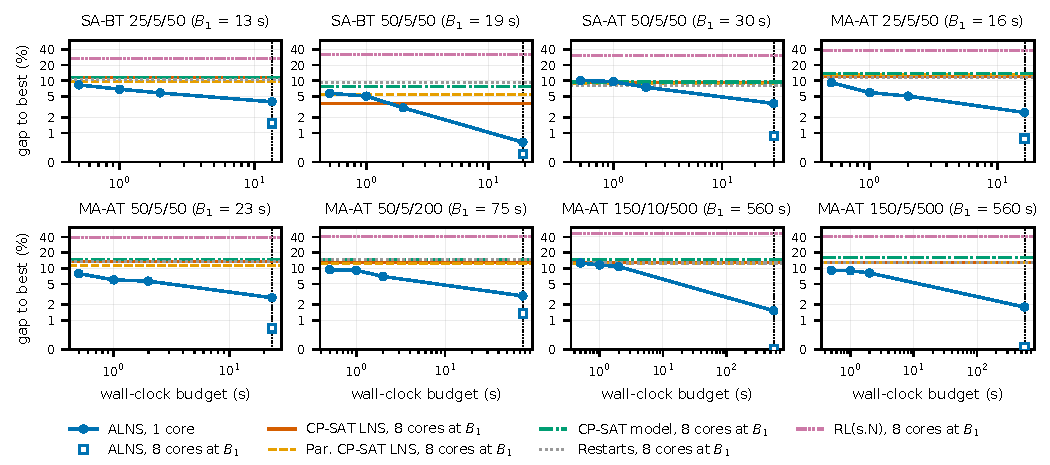
\includegraphics[width=\textwidth]{figures/budget}
\caption{Mean gap to the best known plan (\%, symmetric log scale) against the wall-clock budget. ALNS on one core
(line) at 0.5, 1, 2\,s and $B_1$, and on 8 cores at $B_1$ (open square), against every competitor on 8 cores at $B_1$
(horizontal lines; the dotted vertical line marks $B_1$). CTAS-D, which fails on most instances, is not shown. Test
instances, 50 per setting.}
\label{fig:budget}
\end{figure*}

\paragraph{C1: equal compute.} ALNS on 8 cores is better than every competitor at the same budget $B_1$ on
\ConeBheld{} of the \ConeBsettings{} settings (Table~\ref{tab:ratios}a): \ConeBsig{} of the \ConeBtests{} tests are
significant after Holm's correction (largest adjusted $p = \ConeBmaxp$), and ALNS gives the shorter plan in
\ConeBwon{} of the \ConeBpairs{} paired runs. Its plans are \ConeBclasslo--\ConeBclasshi\% shorter than those of the
three CP-SAT-based methods and greedy restarts, and \ConeBrlgainlo--\ConeBrlgainhi\% shorter than those of the RL
policy.
Settings where C1 does not hold: \ConeBfaillist. The pre-registered decision rule (C1 on at least six of the eight
settings) therefore \ConeBverdict. With twice the budget, $2B_1$, ALNS stays ahead of parallel CP-LNS, CP-SAT full
model and greedy restarts in \ConeBBheld{} of \ConeBBsettings{} settings (\ConeBBsig{} of \ConeBBtests{} tests
significant, plans \ConeBBclasslo--\ConeBBclasshi\% shorter).

\begin{table}[t]
\centering
\small
\caption{Mean gap to the best plan found by any run (\%) and CPU used (CPU seconds of all processes and threads, as a share of 8 cores for $B_1$); range over the eight settings. Every method runs on 8 cores at $B_1$, except ALNS on 1 core for 2\,s. CTAS-D: share of the instances solved within $B_1$, up to 200 tasks.}
\label{tab:methods}
\begin{tabular}{lcc}
\toprule
Method & Gap to best (\%) & CPU used (\%) \\
\midrule
ALNS, 8 cores & 0.0--0.9 & 98--100 \\
ALNS, 1 core, 2\,s & 2.6--10.1 & 0.04--1.7 \\
\midrule
CP-LNS & 3.9--13.8 & 34--79 \\
Parallel CP-LNS & 4.9--13.3 & 97--101 \\
CP-SAT full model & 5.8--16.3 & 51--90 \\
CTAS-D (exact MILP) & solves 0--98\% & 49--96 \\
Greedy restarts & 6.5--14.4 & 97--100 \\
RL policy (published) & 28.3--63.6 & 89--97 \\
\bottomrule
\end{tabular}
\end{table}


\paragraph{Parallelism does not rescue CP-SAT.} CP-LNS uses only \Cpucpsatlo--\Cpucpsathi{} of its 8 cores
(Table~\ref{tab:methods}), because building each subproblem is serial between the multi-threaded solver calls.
Parallel CP-LNS keeps all cores busy (\Cpupcpsatlo--\Cpupcpsathi) and makes many more solver calls
(Table~\ref{tab:steps}), but it is not clearly better: the ratio ALNS / competitor is \ConeBpcpsatlo--\ConeBpcpsathi{}
against the parallel version and \ConeBcpsatlo--\ConeBcpsathi{} against the single search. CP-SAT's own search on the
full model does no better (\ConeBcpfulllo--\ConeBcpfullhi): on the larger instances it rarely improves on the greedy
plan it starts from (in tuning, it ended with that plan on 13 of 16 instances with 200 or 500 tasks). Shorter solver
calls do not help either: with 200 tasks, calls of 0.5\,s or less spent their time building and presolving the
subproblem and never improved the plan in our tuning runs.

\paragraph{The exact MILP.} CTAS-D finds a plan within $B_1$ for \CtasSolved{} of the \CtasRuns{} test instances with
up to 200 tasks (Table~\ref{tab:ratios}a). This matches the published picture, where Gurobi solved few instances of most
50-task settings within an hour \cite{dai2025heterogeneous}: the MILP is a strong method on 20 tasks, where our port
beats the shipped Gurobi solutions, but not a competitor at this scale.

\paragraph{The learned policy.} The RL policy ends \Gaprllo--\Gaprlhi\% above the best known plans, although it
completes \RLNlo{} to \RLNhi{} times the published number of rollouts. Greedy restarts alone give plans
\RestartsRLlo--\RestartsRLhi\% shorter (ratio of means): a careful construction with restarts already closes much of
the gap to the learned policy, and search closes the rest.

\paragraph{C2: one core.} ALNS on a single core for 2\,s is significantly better than every competitor on 8 cores at
$B_1$ on \Ctwoheld{} of the \Ctwosettings{} settings: \Ctwoheldlist{} (Table~\ref{tab:ratios}b;
\Ctwosig{} of \Ctwotests{} tests significant). It does not hold on \Ctwofaillist. Against the learned policy it holds
everywhere, with plans \Ctworlgainlo--\Ctworlgainhi\% shorter than those the RL policy finds on 8 cores in 7 to 280
times the wall-clock time. At 1\,s and 0.5\,s, C2 holds on \CtwoOneheld{} and \CtwoHalfheld{} settings, and at $B_1$
ALNS on one core has a lower mean gap than every 8-core competitor on \OneCoreBoneAhead{} settings (descriptive;
Figure~\ref{fig:budget}).

\paragraph{Scaling with cores.} Eight workers instead of one improve ALNS at $B_1$ by only
\Workersgainlo--\Workersgainhi\% (ratio \Workerslo--\Workershi). Most of its advantage is thus per-core efficiency,
not parallelism.

\paragraph{How good are the plans?} The best known plans on 50 or more tasks come from ALNS runs, which raises the
question whether ALNS is merely close to itself. On the validation instances we ran parallel CP-LNS and CP-SAT full
model for 300\,s on 8 cores, starting from greedy plans only, with 10 to 20 times the compute of $B_1$. On none of the
\RefValInstances{} validation instances with 50 or more tasks did any run without an ALNS component match the best
ALNS-derived plan; the best of them is on average \RefValFreelo--\RefValFreehi\% longer per setting, while ALNS on 8
cores at $B_1$ ends \Gapalnslo--\Gapalnshi\% above the best known plans on the test instances. The certified lower bounds of CP-SAT remain
\RefValBoundlo--\RefValBoundhi\% below the best known plans, so the distance to the optimum is unknown; the paired
ratios above do not depend on it.

\paragraph{Execution.} All \RunsBone{} runs on 8 cores at $B_1$ were scored; \LateBone{} of them overran their budget
by more than 10\% + 0.25\,s and were scored at the budget as pre-registered: \LateRL{} runs of the RL policy, whose
last batch of rollouts can end after the deadline and which keeps no intermediate plan, so that such a run counts as a
failure, \LateALNS{} of ALNS and \LateOther{} of the other competitors. If every late run is instead scored by the
final plan it returned (descriptive, not pre-registered), ALNS's plans are \Sensrlgainlo--\Sensrlgainhi\% shorter
than those of the RL policy. Jobs with more than 40\% throttled CPU periods were re-run and left out; the per-row host conditions are
in the supplement.
